Plan:
\textbf{Two Examples + Algorithm Overview}
\begin{itemize}
\item {Multiple-Path While Loop}
\\
\textbf{The First Challenge/Problem from The Example, 
and the Overview of the New Techniques Targeting This Problem}
\item {Nested While Loop}
\\
\textbf{The Second Challenge/Problem from The Example,
and the Overview of the New Techniques Targeting This Problem}
\end{itemize}
In this section, we discuss two representative examples with
challenges of analyzing the symbolic
\emph{reachability-bound} on
every control location.
We also give the technique overview of our algorithm.
%
\subsection{Multiple-Path Loop}
\label{sec:overview-multiplepath}
\input{examples/whileTwoCounters-overview}
Figure~\ref{fig:whileTwoCounters-overview}(a) shows an example of a two paths loops
with different \emph{reachability-bounds} on the control locations in different paths.
This example is adopted from the example in~\cite{Sumit2010rechability}, which
is a skeleton code from the .Net base-class library.
\\
In this example, given $n \geq m$,
the precise \emph{reachability-bound}s for control locations $4$ and $5$ are both $m \times \lfloor\frac{n}{m}\rfloor$,
for location $2$ and $3$ are $(m + 1) \times \lfloor\frac{n}{m}\rfloor + 1$, 
and $1$ for locations $0, 1$ and $\lex$.
\\
In order to know that the locations in first branch ($4$ and $5$) are reached at most $m \times \lfloor\frac{n}{m}\rfloor$ times
while $6$ in second branch $\lfloor\frac{n}{m}\rfloor$ times
 during program execution,
we need to know that the two if branches are interleaved and executed alternatively after each other
during the iterations of the enclosed loop.
\\
However, to the best of our knowledge, the state-of-art \emph{reachability-bound} computation method~\cite{Sumit2010rechability}
can only give a loop bound $n + \lfloor\frac{n}{m}\rfloor$
as the \emph{reachability-bound} for all the locations inside the loop ($2, 3, 4, 5, 6$), which is loose without considering path-sensitivity.
% There isn't any other work on solving the \emph{reachability-bound} problem.
\\
Among the relevant works about program complexity, cost and loop bound analysis, \cite{GulwaniJK09} can compute the most precise global
loop bound (i.e., $n + \lfloor\frac{n}{m}\rfloor$) for this the loop bound path-sensitively.
Though we can use it as the \emph{reachability-bound} for location $1$ and $2$,
the \emph{reachability-bounds} for control locations $4, 5$ and $6$ are still unclear.
\paragraph{Path reachability-bound}
The first key idea of this path-sensitive \emph{reachability-bound} analysis algorithm is the \emph{path reachability-bound}.
\\
Our algorithm combines the idea of \emph{difference constraint} based program complexity analysis method from \cite{sinn2017complexity}
and the control-flow refinement technique from~\cite{GulwaniJK09} efficiently.
It first
generates the abstract transition graph for the program using the difference constraints, such as Figure~\ref{fig:whileTwoCounters-overview}(b).
Then it transforms every while loop using the control-flow refinement technique from~\cite{GulwaniJK09} and generates a refined program $\rprog$.
% 
The refined program for program $\kw{whileTwoCounters}$ is
\[
  \tpath_0 ; 
  \rpchoose{2: \rprepeat_2(\rprepeat_1(\tpath_1); \tpath_2) , 
  2: \rprepeat_1(\tpath_1) }; \tpath_3,
\]
where the simple transition paths $\tpath_0, \ldots$ are as in Figure~\ref{fig:whileTwoCounters-overview}(c).
Every simple path will not interleave with the others. 
Over the refined program, we first compute the \emph{path reachability-bound} for every simple transition path,
$\inoutB(\rprog, \tpath)$,
which is a bound on the reachability time of $\tpath$ during the execution of $\rprog$.
For this example, the \emph{path reachability-bound} for the three simple transition paths are
$\inoutB(\rprog, \tpath_1) = \max\{m, m \times \lfloor\frac{n}{m}\rfloor\}$ \quad
$\inoutB(\rprog, \tpath_2) = \lfloor\frac{n}{m}\rfloor$ \quad
$\inoutB(\rprog, \tpath_0) = \inoutB(\rprog, \tpath_3) = 1$.
\\
Then we use this bounds
and another \emph{loop reachability-bound}
to compute the final \emph{reachability-bound} for each location.
Since there isn't nested loop in this example, we simply sum up $\inoutB(\rprog, \tpath)$ over the $\tpath$ where a certain location shows up
and as its \emph{reachability-bound}.
%  and compute the expected bound for each location.
%
\subsection{Nested Loops with Related Iterator}
\label{sec:overview-nestedwhile}
However, when there exists nested loop, computing the \emph{reachability-bound} for each location encounters another challenge.
Though we have
%  local 
the \emph{reachability-bound} for every transition path, which is not precise enough in nested loop.
Figure~\ref{fig:threeWhile-overview}(a) shows an example of the nested loops with related 
iterators.
This example is adopted from the example in~\cite{GulwaniJK09}, which is common in product code.
\\
In line 8, $i$ is reset by $w$ and $w$ is reset by $j$ at line 5. So the
while $L_6$ is only executed in the first iteration of while loop $L_1$ and $L_3$.
% \\
The while loop $L_3$ at line 3 is executed only in 
the first $m - N$ iterations of the 
$L_1$ because $j$ is reset by $i$ in line 2.
% \\
So the total combined iterations of all the three loops is bounded above by 
$n + m^2 - m \times N$,
and the precise \emph{reachability-bound} for location $7$ inside the $L_6$ is $N$,
for locations $4, 5$ and $8$ between the $L_3$ and $L_6$ are $(n-N) \times (m - N)$,
and $n - N$ for locations $2$ and $9$.
\\
\highlight{Notice here the global \emph{reachability-bounds} for the locations inside the loop $L_6$ is 
the same as its loop iteration bound, as well as our \emph{path reachability-bound}.
However, for the locations between $L_3$ and $L_6$,
the \emph{reachability-bounds} are the multiplication of the inner and outer loop iteration bounds.}
\\
So far, the loop bound analysis method in \cite{GulwaniJK09} can only give a loose bound $n + (m \times n) + N$ for the entire loop complexity, and 
the DC-based algorithm in \cite{sinn2017complexity} is able to
compute a better combined loop bound of $n + m^2 - m \times N$ but still loose.
\\
None of the state-of-art methods can give the precise \emph{reachability-bounds} for every location in these nested loops.
\\
And it is not trivial to compute the \emph{reachability-bound} for every locations in nested loops even though knowing the loop bound,
especially the locations which are similar to $7$ in $\kw{threeNestedWhile}$.
\\
\highlight{
In order to precisely compute how many times the location $7$ is reached, we need to know
the numbers of iterations of the outside loop $L_3$ and $L_1$, 
during which the loop $L_6$ is entered. 
We call this the \emph{loop reachability} of the loops $L_3$ and $L_1$ w.r.t to the location $7$, and we multiply the loop bounds of the $L_6$ with the \emph{loop reachability} where $L_6$ is nested to get the precise
\emph{reachability-bounds} for location $7$.
}
\\
\highlight{
This quantity isn't considered or computed in any of the previous works.
The \emph{Progress Invariant} method in \cite{GulwaniJK09} is only able to compute
the
bound on iteration numbers
of the inner loop $L_6$ in each iteration of $L_3$ and $L_1$, which are both $N$.
So they have to over-approximate the reachability-bound for locations inside $L_6$ with the
overall program complexity, i.e., $n + m^2 - m \times N$.
\\
For the same reason, the DC-based algorithm in \cite{sinn2017complexity}
is only able to
compute the precise combined loop bound and the local bound of each loop
separately as well.
We are still unable to know the precise \emph{reachability-bound} for the locations in the innermost loop.
}
\paragraph*{Loop reachability-bound.}
The second key idea of our path-sensitive reachability analysis algorithm is the
\emph{loop reachability-bound} for each transition path $\tpath$ w.r.t a loop where it is nested,
$\lpchB(L:\rprog, \tpath)$.
\highlight{It is a bound on the iterations for
the outside $L:\rprog$ w.r.t. the innermost loop where $\tpath$ is enclosed.
Such that during these iterations of $L:\rprog$, the innermost loop is entered. 
This is distinguished from the traditional methods, which only compute the bound on the inner loop's maximum iteration number
in one iteration of the outside loop.}
\\
For this example, we first generate its abstract transition graph as well in Figure~\ref{fig:threeWhile-overview}(a),
and then computes its refined program,
$\rprog = \tpath_0; 1: \rprepeat(\tpath_1;$ 
$3: {\rprepeat(\tpath_2; 6 : {\rprepeat(\tpath_3)}; \tpath_4)}; \tpath_5);$ 
$\tpath_6$,
where the $\tpath_0, \ldots$ are shown below the graph in Figure~\ref{fig:threeWhile-overview}(b).
We use $\rprog_1$ to denote ${\rprepeat(\tpath_1; 3: {\rprepeat(\tpath_2; 6 : {\rprepeat(\tpath_3)}; \tpath_4)}; \tpath_5)}$
and $\rprog_3 = {\rprepeat(\tpath_2; 6 : {\rprepeat(\tpath_3)}; \tpath_4)}$
for simplicity.
Then we compute \emph{loop reachability-bound} for these simple paths w.r.t. each of their nested loop.
For example, for $\tpath_3$ w.r.t. the loop $L_1$ and $L_3$, we compute
$\lpchB(1: \rprog_1, \tpath_3) = 1$ and
$\lpchB(3: \rprog_3, \tpath_3) = 1$ because loop $L_6$ will only be entered once among all iterations of $L_1$ and $L_3$.
% $\lpchB(3: \rprog_3, \tpath_3) = 1$
% means that during all iterations of the loop at $1$, there is only $1$ iteration where the loop at $6$
% (the closest loop enclosing $\tpath_3$) is executed.
Among all the other $n - 1$ iterations of $L_1$, the loop $L_6$ isn't executed at all.
So we compute the \emph{loop reachability-bound}  of the loop $L_3$
w.r.t to this path is $1$.
In the same way, we also compute $\lpchB(3: \rprog_3, \tpath_3) = 1$ precisely.
Then we sum up the bound of the path where each location shows up
and as its \emph{reachability-bound} still as before,
and multiply this result by all its \emph{loop reachability-bound}s.
In this way, we compute $N$ as the \emph{reachability-bound} of location $7$, which is tight.
    %
    \begin{figure}
    \centering
    %
    \begin{subfigure}{.45\textwidth}
        $
        \begin{array}{l}
            N < m < n\\
            \kw{threeNestedWhile}(n, m, N) \triangleq \\
            \clabel{ \assign{i}{0} }^{0} ; \\
                L_1: \ewhile ~ \clabel{i < n}^{1} ~ \edo ~ \\
                \quad \Big(
                 \highlight{\clabel{\assign{j}{0}}^{2}} ;\\
                 L_3:  \quad \ewhile ~ \clabel{j < m}^{3} ~ \edo ~ \\
                \quad \quad \Big( \clabel{\assign{j}{j+1}}^{4};\\
                  \quad \quad \highlight{\clabel{\assign{w}{i}}^{5}};\\
                  L_6:  \quad \quad \ewhile ~ \clabel{w < N}^{6} ~ \edo ~ \\
                  \quad \quad \quad \Big( \clabel{\assign{w}{w + 1}}^{7}
                      \Big); \\
                      \quad \quad \clabel{\assign{i}{w}}^{8}
                      \Big); \\
                      \quad \clabel{\assign{i}{i+1}}^{9}
                  \Big)
            \end{array}
            $
    \caption{}
        \end{subfigure}
    \begin{subfigure}{.48\textwidth}
        \begin{centering}
            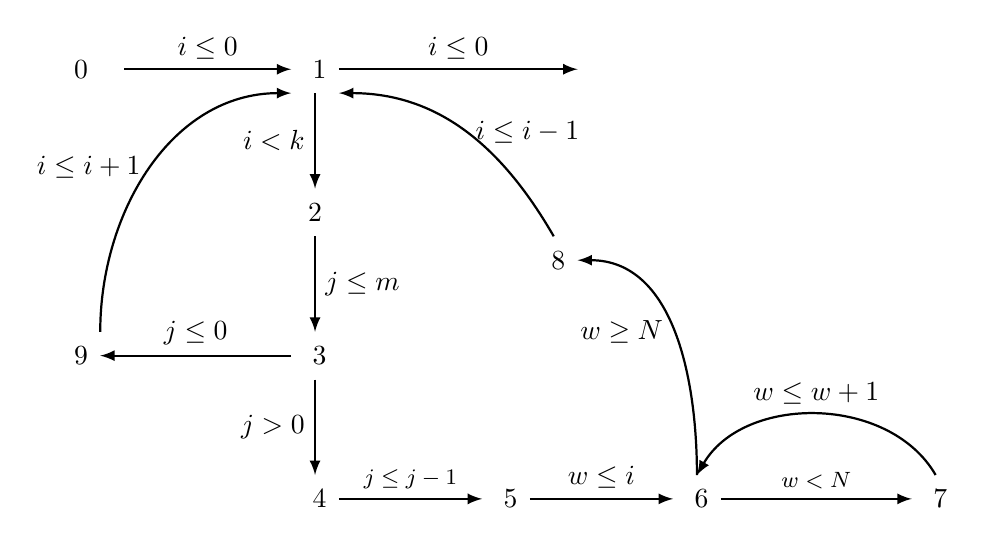
\begin{tikzpicture}[scale=\textwidth/20cm,samples=200]
                \draw[] (-5, 10) circle (0pt) node{{ $0$}};
                \draw[] (0, 10) circle (0pt) node{{ $1$}};
                \draw[] (6, 10) circle (0pt) node {{$\lex$}};
                \draw[] (0, 7) circle (0pt) node{{$2$}};
                \draw[] (0, 4) circle (0pt) node{{ $3$}};
                \draw[] (-5, 4) circle (0pt) node{{ $9$}};
                \draw[] (0, 1) circle (0pt) node{{ $4$}};
                \draw[] (4, 1) circle (0pt) node{{ $5$}};
                \draw[] (8, 1) circle (0pt) node{{ $6$}};
                \draw[] (13, 1) circle (0pt) node{{ $7$}};
                \draw[] (5, 6) circle (0pt) node{{ $8$}};
                % Counter Variables
                %
                % Control Flow Edges:
                \draw[ thick, -latex] (-4, 10)  -- node [above] {$i \leq 0$}(-0.5, 10);
                \draw[ thick, -latex] (0, 9.5)  -- node [left] {$i < k$} (0, 7.5) ;
                \draw[ thick, -latex] (0, 6.5)  -- node [right] {$j \leq m$} (0, 4.5) ;
                \draw[ thick, -latex] (0, 3.5)  -- node [left] {$j > 0$} (0, 1.5) ;
                \draw[ thick, -latex] (-0.5, 4)  -- node [above] {$j \leq 0$} (-4.5, 4) ;
                \draw[ thick, -latex] (-4.5, 4.5)  to  [out=90,in=180]  node [left] {$i \leq i + 1$ }(-0.5, 9.5);
                \draw[ thick, -latex] (0.5, 10)  -- node [above] {$i \leq 0$}  (5.5, 10);
                \draw[ thick, -latex] (0.5, 1)  -- node [above] {{\footnotesize $j \leq j - 1$}}  (3.5, 1);
                \draw[ thick, -latex] (4.5, 1)  -- node [above] {$w \leq i$}  (7.5, 1);
                \draw[ thick, -latex] (8.5, 1)  -- node [above] {{\footnotesize $w < N$}}  (12.5, 1);
                \draw[ thick, -latex] (8, 1.5)  to [out=90,in=0] node [left] {{$w \geq N$}}  (5.5, 6);
                \draw[ thick, -latex] (13, 1.5)  to  [out=120,in=60] node [above] {$w \leq w + 1$}  (8, 1.5);
                \draw[ thick, -latex] (5, 6.5)  to  [out=120,in=0]  node [right] {$i \leq i - 1$ }(0.5, 9.5);
                \end{tikzpicture}
%     \caption{}
%     \end{centering}
%     \end{subfigure}
% \begin{subfigure}{.2\textwidth}    
% \begin{centering}
    {\small
$
    \begin{array}{ll}
        \tpath_0 = (0 \to 1)
        &
        \tpath_4 = (6 \to 8 \to 3)
        \\        
        \tpath_1 = (1 \to 2 \to 3)
        &
        \tpath_5 = (3 \to 9 \to 1)
        \\
        \tpath_2 = (3 \to 4 \to 5 \to 6)
        &
        \tpath_6 = (1 \to \lex)
        \\
        \tpath_3 = (6 \to 7 \to 6)
    \end{array}
$
$
    \begin{array}{l}
        \rprog_1 = {\rprepeat(\tpath_1; 3: {\rprepeat(\tpath_2; 6 : {\rprepeat(\tpath_3)}; \tpath_4)}; \tpath_5)}
        \\
        \rprog_3 = {\rprepeat(\tpath_2; 6 : {\rprepeat(\tpath_3)}; \tpath_4)}
    \end{array}
$
}
\caption{}
\end{centering}
\end{subfigure}
    \caption{
    (a) An example of three nested loops with related iterator variables.
    (b) The abstract transition graph, simple transition paths and loop body.}
        \label{fig:threeWhile-overview}
    \end{figure}
